
\documentclass[
letterpaper,
11pt,
%answers,
]{exam}

\usepackage[lmargin=0.75in,rmargin=0.75in,tmargin=1in,bmargin=1in]{geometry}
\usepackage{enumitem}
\usepackage{graphicx}
\usepackage{tikz}
\usepackage{multicol}

% Sets the column separation so that enumeration doesn't cause
% the line between columns interfere with the numbers.
\setlength{\columnsep}{4em}

%\setlength{\columnseprule}{0.4pt}

% Code block creates the Matching question format
\newcommand*\Matching[1]{
\ifprintanswers
\textbf{#1}
\else
\rule{2.5in}{0.5pt}
\fi
}
\newlength\matchlena
\newlength\matchlenb
\settowidth\matchlena{\rule{2.5in}{0pt}}
\newcommand\MatchQuestion[2]{%
\setlength\matchlenb{\linewidth}
\addtolength\matchlenb{-\matchlena}
\parbox[t]{\matchlena}{\Matching{#1}}\enspace\parbox[t]{\matchlenb}{#2}}

% Formats the header on the first page where the student enters their name and date.
\newcommand{\head}{%
\thispagestyle{empty}
\vspace*{-0.75in}
\noindent
\class \hfill Name \makebox[7cm]{\hrulefill}\par
\vspace{10pt}
\noindent
\Large\textbf{\wstitle}\normalsize \hfill Date \makebox[3.5cm]{\hrulefill}Ver: \wsVer\par
\vspace{10pt}
}

% Defines the titles and instructions for the worksheet or test
\newcommand{\class}{Humanities IV}
\newcommand{\wstitle}{Experiment Number 30}
\newcommand{\wsVer}{5}
\newcommand{\Instructions}{Identify each region marked.}

% Sets the running header at the top of the subsequent pages
\pagestyle{head}
\runningheader{\class\ \wstitle}{}{Page \thepage\ of \numpages}

% BEGINNING OF DOCUMENT
\begin{document}
\head
\setlength{\linewidth}{7in}

% Display the map/image with the labels applied
\noindent
\begin{tikzpicture}
    % Include the image
    \node[anchor=south west,inner sep=0] at (0,0) {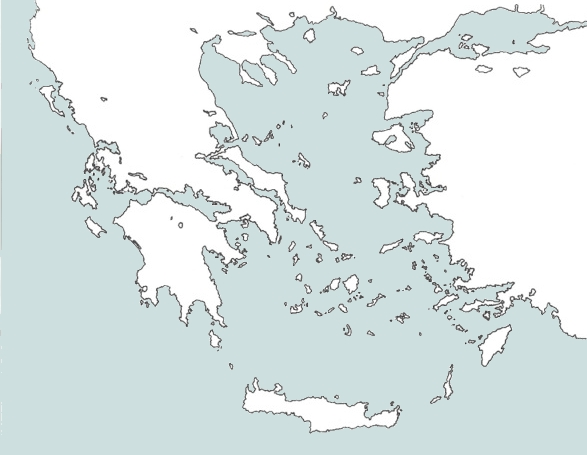
\includegraphics[width=\textwidth]{/home/jon/Documents/Coding/MapQuizMaker/blankGreekmap.jpg}};

    % Overlay text at specific coordinates
    %\node at (1, 1) {\textbf{LABEL}};  % (1, 1) is location (in cm) of LABEL on the map/image
    \node at (12.4, 11.3) {\textbf{1}};
\node at (5.2, 8.8) {\textbf{2}};
\node at (14.4, 6.9) {\textbf{3}};
\node at (10.2, 9.0) {\textbf{4}};
\node at (10.1, 1.1) {\textbf{5}};
\node at (5.2, 6.2) {\textbf{6}};
\node at (8.0, 7.3) {\textbf{7}};

\end{tikzpicture}
%}

\noindent
\textit{\Instructions}\par
%\textit{Fill in each blank with the name corresponding to the number on the map.}\par

\begin{questions}

\begin{multicols}{2}
    % \question\MatchQuestion{ANSWER}{PROMPT} \vfill
    \question\MatchQuestion{Troy}{} \vfill
\question\MatchQuestion{Boeotia}{} \vfill
\question\MatchQuestion{Ionia}{} \vfill
\question\MatchQuestion{Aegean}{} \vfill
\question\MatchQuestion{Krete}{} \vfill
\question\MatchQuestion{Pelopponese}{} \vfill
\question\MatchQuestion{Attika}{} \vfill
\end{multicols}

\end{questions}
\end{document}